\documentclass{article}
\usepackage[utf8]{inputenc}
\usepackage{graphicx}
\usepackage{titlepic}
\usepackage{caption}
\usepackage{subcaption}
% \documentclass{beamer}

\newcommand{\namesigdate}[2][5cm]{%
  \begin{tabular}{@{}p{#1}@{}}
    #2 \\[0.4\normalbaselineskip] \hrule \\[0pt]
    {\small } \\[2\normalbaselineskip] 
  \end{tabular} 
}

\title{\textbf{Hybrid Logical Clocks}}
\author{Vaibhav Bhagee (2014CS50297)}
\date{}

\begin{document}
\maketitle

\begin{center}
\noindent\rule{3.2cm}{0.4pt} 
\end{center}

    \section{Introduction}

    Ordering of events in a distributed system is of utmost importance when arguing about causality and correctness, with clocks lying at the very heart of that. Most of the work done in distributed computing completely disregards the physical notion of time and is based on its logical notion. While that helps us track causality of events in a system, most physical implementations can't entirely do away with the physical notion of time in order to support real time operations and queries. \\

    Physical clocks are also known to have issues, related to non monotonosity and drift, which makes them infeasible for causality tracking. In this report, we look at Hybrid Logical Clocks\cite{hlc}, which help us get the best out of both worlds. HLC timestamps enable tracking causality of events in a distributed system, while being a bounded approximation to the system time. Further properties of HLCs along with their applications, have been discussed is greater detail in the subsequent sections.

    \section{Motivation}

    There have been various attempts made towards formulation of algorithms, used to timestamp events in a distributed system. A key requirement from such an algorithm is that the timestamps should be such that they should at least enable tracking causal dependencies among the events of the system. \\

    Let us denote the timestamp of an event $e$ as $t.e$. Then, in particular, for two events $e$ and $f$, $$e \prec f \rightarrow t.e < t.f$$ where $\prec$ is the $happens\ before$ relation.

    \subsection{Logical and Vector Clocks}

    Logical clocks\cite{lc} proposed by Lamport and Vector clocks\cite{vc} proposed by Mattern, timestamp the events based on the logical notion of time. They do away with system clocks and the physical notions of time. Both the algorithms enable tracking of causal dependencies as described above. Vector clocks further ensure that for two events $e$ and $f$, $$e \prec f \iff t.e < t.f$$ where $\prec$ is the $happens\ before$ relation. \\

    However, real time deployments of distributed systems cannot rely solely on logical and vector clocks. Many systems like distributed databases require answering of queries which rely on physical time. An example of such a query in a system which tracks jobs running on a group of virtual machines could involve returning the IDs of the events which failed in the part hour. In such a scenario, logical clocks become incapable of answering such queries. \\

    Also, vector clocks have an associated space overhead, where the storage is proportional to the number of processes in the system. Many algorithms have since been proposed which try to bound the storage of the vector clock timestamps. While those algorithms successfully bound the storage costs, the trade of has to be made with an increased computation cost, while tracking the causal dependencies.

    \subsection{Physical Clocks}

    Physical clocks, unlike logical clocks, take into account the system time at the nodes. The vanilla physical clocks suffer from issues of $drift$ and $non\ monotonosity$. Due to the different rates at which the clocks at different nodes of the system might tick, the latter may eventually drift apart. This leads to a periodic requirement for $clock\ synchronisation$. \\

    While synchronisation resolves the problem of drift, it leads to a new problem of non monotonosity. Due to the periodic synchronisation, it may so happen that the timestamp at a later stage of the protocol, might turn out to be lesser that the timestamp at an earlier stage. Thus, it can happen that for two events $e$ and $f$, the event $e\ \prec\ f$ but $l.e\ >\ l.f$. This leads to periods of uncertainty and subsequently leading to inability to order events.

    \subsection{True Time}

    True time is proposed by Google, as a part of their strongly consistent distributed database called Spanner\cite{spanner}. Spanner utilises GPS and atomic clocks for tight clock synchronisation. This leads to a very low clock drift. However, this can still have small periods of uncertainty. True time, exposes this uncertainty as an abstraction. \\

    The timestamp allotted by True time is a tuple $(earliest,\ latest)$, which specifies the bounds in which the exact timestamp could lie. If the intervals for two events overlap, it leads to uncertainty. To overcome this limitation, Spanner uses the idea of inducing delays. This means that if an event $e\ \prec\ f$ and the timestamps of $e$ and $f$ are not disjoint, then we delay $f$ to a point where $f.earliest\ >\ e.greatest$. \\

    To overcome the limitations of the algorithms, as pointed out earlier, the authors propose Hybrid Logical Clocks.

    \section{Hybrid Logical Clocks}

    For every event $e$, the HLC associates a timestamp value $t$ such that $t\ =\ (l,c)$. Here $l$ is the physical component of the timestamp and $c$ is the logical component. While preserving the causal ordering property of logical clocks, the HLC timestamps are withing an $\epsilon$ bound of the physical clock timestamps. The updates to the HLC timestamps are monotonic and the space requirement for the HLC timestamp is bounded.

    \subsection{Algorithm}

    At an abstract level, for an event $f$, the HLC timestamp at $f$ depends on the HLC timestamp at the predecessor(s) of $f$. If the physical clock timestamp at the event $f$ has not caught up with the value of the physical component of the HLC timestamp at the predecessor, then the causal component of the HLC timestamp at $f$ is incremented by 1, to capture the causality while the physical component of the latter is kept equal to the corresponding component of the predecessor. However, if the physical timestamp at $f$ manages to catch up, as discussed before, then the causal component gets reset to 0. A formal algorithm is given in figure 1. 

    \begin{figure}[h!]
        \begin{center}
        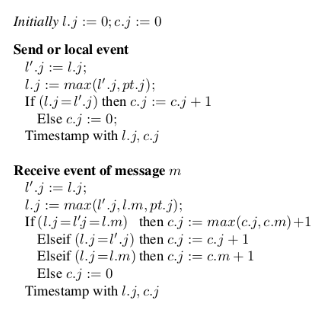
\includegraphics[resolution=125]{algorithm.png}
        \end{center}
        \caption{HLC Algorithm}
    \end{figure}

    \subsection{Properties}

    After having looked at the HLC algorithm, we will now look at the properties satisfied by the HLC timestamps. We will discuss about the reasoning in brief. The interested readers can take a look at the technical paper, for the detailed arguments. \\

    \noindent \textbf{Theorem 1:} For any two events $e$ and $f$, $$e \prec f \rightarrow (l.e,c.e) < (l.f,c.f)$$ \\

    This can be formally proved, directly from the algorithm. Intuitively, if $e\ \prec\ f$, then due to the use of the $max$ function, we can show that $l.e\ \leq\ l.f$. Now, if $l.e\ <\ l.f$ then the consequent becomes true. Otherwise if $l.e\ =\ l.f$ then, by the algorithm, $c.f\ =\ c.e\ +\ 1$. \\

    \noindent \textbf{Theorem 2:} For any event $f$, $l.f\ \geq\ pt.f$ \\

    This is also a direct consequence of the algorithm. \\

    \noindent \textbf{Theorem 3:} $l.f$ denotes the maximum clock value that $f$ is aware of. Thus, $$l.f > pt.f \rightarrow (\exists g: g \prec f \land pt.g = l.f)$$ \\

    This can be proved using induction. For the induction step, we consider the cases when $f$ is a send event or a receive event. In the former case, let $e$ be the event just preceding the send. Thus, for $e$ we have $$l.e > pt.e \rightarrow (\exists g: g \prec e \land pt.g = l.e)$$ Now, if $l.f\ >\ pt.f$, then, according to the algorithm, we have $l.e\ =\ l.f\ =\ pt.g$. The proof for the latter case is similar to the proof of the former. \\

    \noindent \textbf{Theorem 4:} For any event $f$, $|l.f\ -\ pt.f|\ <\ \epsilon$ \\

    We use the clock synchronisation constraints for the physical clocks, which ensure that there cannot exist events $g$ and $f$ such that $g\ \prec\ f$ and $pt.g\ >\ pt.f\ +\ \epsilon$. Also, using the previous theorem we have $$l.f > pt.f \rightarrow (\exists g: g \prec f \land pt.g = l.f)$$ But, $pt.g\ \leq\ pt.f\ +\ \epsilon$. Thus, $l.f\ \leq\ pt.f\ +\ \epsilon$. \\

    \noindent \textbf{Theorem 5:} For any event $f$, $c.f\ =\ k\ \land\ k\ >\ 0\ \rightarrow$ $\exists$ a chain of $k$ events which causally precede the event $f$ in the system, having the same value of the physical component of the HLC. \\

    This property is similar to the property of Lamport clock timestamps. This can be proved using induction, as the authors have suggested in the paper. Intuitively, we can again split the proof into cases when $f$ is a send or a receive event and both the cases are proven similarly. For the send case, let $e$ be the event which causally precedes $f$. Then, if $l.e\ =\ l.f$, we have $c.f\ =\ c.e\ +\ 1$ and $e$ satisfies the induction hypothesis. As mentioned, the proof of the case when $f$ is a receive event, is similar. \\

    \noindent \textbf{Theorem 6:} For any event $f$, $c.f\ \leq\ N*(\epsilon\ +\ 1)$ \\

    This proof can be done using the clock synchronisation constraints again. Using the constraints, we can conclude that for all events $e$ having $l.e\ =\ l.f$, the event would have happened at a physical time lying in $[l.f,\ l.f+\epsilon]$. Also, at any node, the number of events which can happen in this time interval is at most $\epsilon\ +\ 1$. This is due to the constraint that the physical clock gets incremented by at least $1$ between two subsequent events on the same node. Hence, for $N$ processes, the bound becomes $N*(\epsilon+1)$. \\

    \section{Applications of HLCs}

    \subsection{Consistency in distributed databases}

    Before going into the discussion about consistent reads and writes in a distributed database deployment, lets us first take a look at the ACID properties, which are satisfied by transactions on relational databases. \\

    \noindent \textbf{Atomicity:} The transactions should happen in an atomic fashion i.e, they should either complete or in case of errors, should leave the database in a state where they appear to have never happened.\\

    \noindent \textbf{Consistency:} The database should go from one consistent state to another, after a transaction. In terms of reads and writes, if a value $x$ is updated in a transaction $T$ by a write operation $w$, then for all the read operations on $x$ which happen after $w$ but before any other write, the value returned should be the one written by $w$. \\

    \noindent \textbf{Isolation:} Transactions can happen in a concurrent fashion but the final state should be such that it should be reachable from the initial state by a sequential application of the participating transactions. \\

    \noindent \textbf{Durability:} Once a transaction is committed, the changes should be persistent. \\

    Distributed database deployments, in order to satisfy the ACID properties, need to make a trade off with efficiency. In order to update all the replicas with the written value, concurrent writes or concurrent read with a write need to be sequenced, leading to a loss off efficiency and speed. \\

    A cluster may decide to reflect the updates on each of the replicas before marking the write as committed, as in the case of $strict\ consistency$ or it may mark the write as committed once the changes are made on the master, while deferring the updates on the other replicas, as in the case of $eventual\ consistency$.

    \begin{figure}[h!]
        \begin{center}
        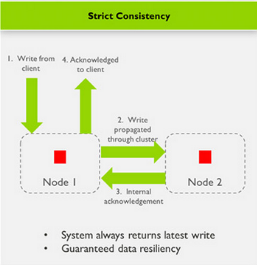
\includegraphics[resolution=125]{strict_consistency.png}
        \end{center}
        \caption{Strict consistency}
    \end{figure}

    \begin{figure}[h!]
        \begin{center}
        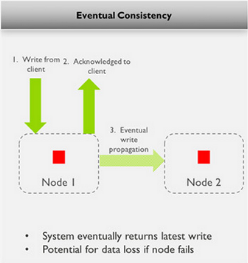
\includegraphics[resolution=125]{eventual_consistency.png}
        \end{center}
        \caption{Eventual consistency}
    \end{figure}

    However, eventual consistency has the problem of stale reads. If a read happens from a replica where the write has not yet been reflected, it leads to the read returning an old value. This can lead to issues if the application is a sensitive one, like banking. \\

    In order to ensure strict consistency without compromising much on efficient, many data bases make use of $multi\ version\ concurrency\ control$. 

    \begin{figure}[h!]
        \begin{center}
        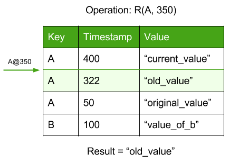
\includegraphics[resolution=125]{mvcc.png}
        \end{center}
        \caption{MVCC}
    \end{figure}

    In MVCC, multiple timestamped versions of the object are maintained in the database, where timestamp denotes the last time at which the object was read. If a write intends to update the value of an object, it first checks if the latest timestamp associated with the object is not more than the timestamp of the write. If that is the case, the transaction gets aborted. Otherwise, a new copy of the object is created with the write timestamp as the timestamp of the write which is being performed and added to the database. For reads, that copy of the object which has the highest write timestamp just lower than the read timestamp, is read. \\

    Hybrid Logical Clocks are used to timestamp the these objects. Since the timestamps preserve causality while being within a bound of the physical time, they allow the database reads to be consistent and alongside that, retaining the information about the physical time, ensuring that queries relying on system time can also be performed.

    \subsection{Global snapshotting}

    In global snapshotting with logical clocks, an initiator process had to take charge of the initiation of the algorithm, while passing around messages for identification of consistent cuts. What prevented every process to take independent charge of taking the snapshot of its system state at a fixed time was the fact that there was no notion of physical time available to the processes and the logical time at multiple processes could be the same for vastly different physical times. \\

    HLC timestamps can be used to ensure that if all the processes take a snapshot of their state at a fixed HLC timestamp say $k$, then these snapshotting events are bound to be concurrent, always leading to consistent cuts. Moreover, a snapshot taken at a process, at an HLC timestamp of $(l=k,c=0)$ will always be a good estimate of the system state at physical time $k$, due to the properties of HLCs discussed above.

    \section{Extensions and research directions}

    \subsection{Event ordering and predicate detection}

    HLCs can be integrated with event ordering services, like Kronos\cite{kronos}, where every process could register the occurrence of an event at an HLC time $t$, with the ordering service, and the same could be locally performed at every process at the specified time. The results could later be collected by the monitor processes and used. This essentially makes the problems like snapshotting, predicate detection, termination detection etc. local operations to an extent, avoiding multiple rounds of message passing to ensure consistency and correctness.

    \subsection{Physical time with vector clocks}

    The current limitation of HLC is that if for events $e$ and $f$ we know that $hlc.e\ <\ hlc.f$ then we can conclude that either $e\ \prec\ f$ or $e$ and $f$ were concurrent. If, we can integrate the ideas of vector clocks with physical time in a way which can also ensure that $hlc.e\ <\ hlc.f$ if and only if $e\ \prec\ f$, then we could use this modified clock algorithm in consensus protocols involving some kind of leader election, to impose a total order on the requests made by the individual processes, at a global level, and choose the minimum one as the leader, thereby avoiding multiple rounds of message passing.

    \newpage

\bibliographystyle{acm}
\bibliography{references}

\end{document}